\chapter{Implicações para aprendizagem científica}

O desenvolvimento da computação e o amadurecimento da noção de pensamento computacional traz consigo várias implicações e oportunidades educacionais.

De partida, pode-se dizer que a efetivação do uso do computador como ferramenta para resolução de problemas exige a formação de capital humano. Normalmente, espera-se que estudantes tenham acesso à universidade para introdução das primeiras noções de programação e ciência da computação. Sabe-se contudo que eles se mostram cada vez familiarizados com \textit{smartphones} e outros dispositivo computacionais. Por isso podemos nos perguntar: por que não antecipar essa instrumentalização? 

Esse questionamento se torna ainda mais pertinente em face do percentual reduzido de portadores de grau universitário. A demanda por profissionais com experiência na resolução de problemas computacionais tem crescido numa proporção superior a que academia tem formado. Esse desequilíbrio tem levado grandes empresas de tecnologia como o Google e IBM a dispensar a formação universitária como pre-requisito para contratação \cite{Purtill}.

A motivação para essa antecipação não é apenas de caráter laboral. Como discutiremos ao longo desse capítulo o uso de computadores e do pensamento computacional oferece excelentes contextos para desenvolvimento de competências científicas. O reverso também é verdadeiro: problemas científicos e matemáticos são domínios excelentes para a aplicação e exercício do pensamento computacional. É nessa tese que esse trabalho se apoia. 

No capítulo \ref{pensamento-computacional} mostramos o como conceitos de abstração, decomposição de problemas e simulação, aliados a praticas de representação de problemas se estruturam em torno do pensamento computacional. Ao mesmo tempo que são centrais na ciência do computação, estes elementos também são fundamentais para o desenvolvimento de modelos e para a compreensão e resolução de problemas num largo espectro de disciplinas matemáticas e científicas \cite{Sengupta2013}.

% Soloway argumenta que aprender a programar corresponde a aprender construir mecanismos e explicações. Portanto a capacidade de construir modelos computacionais por programação corresponde a 

A literatura tem demonstrado de diversas formas o como a aprendizagem de programação - uma das praticas de representação - em conjunto com conceitos de outros domínios pode ser mais fácil do que aprender cada um desses tópicos individualmente. Essa abordagem é destacadamente diferente da forma como o ensino de computação tem sido trabalhado no ambiente escolar, onde as atividades propostas focam em aspectos apartados da realidade.

Em um estudo citado por \citeonline{Weintrop2016}, descobriu-se que a introdução de programação no contexto da modelagem de fenômenos físicos e químicos, durante as atividades de alunos de graduação, resultaram no aprendizado mais efetivo de programação, e no aumento do engajamento com a área de domínio das tarefas.

A literatura também nos apresenta outros exemplos de contextualização de atividades computacionais com o ensino de ciências. Dentre algumas propostas práticas, podemos destacar o uso eficiente do software Netlogo \cite{netlogo} na introdução de noções de probabilidade e estatística, como relatado por \citeonline{ProbLab}, e na modelagem de fenômenos epidemiológicos, tal como reportado em \cite{Lee:2011:CTY:1929887.1929902}.

% O enriquecimento das atividades em sala dae aula não tem sido o único
Vários estudos apontam que o enriquecimento trazido por essa abordagem conjunta, associada com o caráter ``mão na massa'' de muitas dessas atividades, produz impactos positivos na forma como os alunos percebem as aulas de ciências \cite{Lee:2011:CTY:1929887.1929902, Barr2011}. A sensação de estar resolvendo um problema autêntico com real aplicabilidade e, em muitos casos, inserido na realidade do qual fazem parte, produz aumentos sensíveis dos níveis de engajamento.

\citeonline{Weintrop2016} sugere que o aumento da atratividade dessas disciplinas, apresentadas dessa forma, também pode favorecer o aumento da representação de grupos minoritários nos meios científicos, tais como mulheres, negros e transgêneros.

A atenção crescente que educadores têm dado ao tema do pensamento computacional tem sido apoiado também pela expectativa de inverter a relação entre os estudante e a tecnologia. A pergunta que se coloca é: como de meros usuários eles podem vir a tornar criadores? 

\citeonline{resnick} argumenta que apesar de serem vistos como ``nativos digitais''\footnote{A expressão ``nativo digital'' foi cunhada pelo escritor Marc Prensky para designar aqueles que desde o seu nascimento tiveram a oportunidade de interagir com tecnologias digitais, tais como videogames, computadores, telefone celular, iPhones, iPads...},  a geração nascida durante esse século esta familiarizada apenas com o consumo de tecnologia, e não necessariamente com a sua criação ou produção. Para ele, o beneficio de dotá-la com essa capacidade criativa não estará apenas nessa ou naquela tecnologia desenvolvida pelo estudante, mas sim nas competências cognitivas adquiridas por ele durante o processo de criação. Dentre algumas delas, o autor destaca:

\begin{enumerate}
  \item a capacidade de pensar em termos sistêmicos, ou seja, em função do comportamento agregado resultante da interação dos componentes de sistema - ``o todo não é a soma das partes''; 
  \item a habilidade para trabalhar em equipe;
  \item a competência para estruturar e planejar as etapas de um projeto;
  \item a facilidade para experimentar novas ideas (prototipagem); 
  \item a destreza para decompor ideias complexas em unidades menores (abstrações);
  \item a perícia necessária para investigar defeitos ou comportamentos inesperados (depuração);
  \item a inteligência emocional necessária para lidar com frustrações e perseverar em face de dificuldades que surgem ao longo de um projeto.  
\end{enumerate}

Como ressalta, mesmo que o estudante não venha a se tornar um engenheiro ou um cientista da computação todas essas competências são importantes para todo e qualquer tipo de atividades. Analogamente, mesmo que poucos deles se profissionalizem como escritores, a capacidade para redigir textos é fundamental para qualquer um.

\citeonline{resnick} direciona o seu argumento para justificar os benefícios do ensino de programação. Veremos, contudo, que o desenvolvimento dessas competências criativas - todas elas associadas ao pensamento computacional - podem passar por caminhos diferentes da habilidade de escrever código, propriamente dita. 

Outras oportunidades educacionais estão associadas às respostas que essa abordagem oferece para vários problemas relacionados ao tema da avaliação. O ensino de ciências é dominado por uma tradição explicativa cujo objetivo é a simples transmissão de dados e conceitos pelo professor. Nesse contexto, convencionou-se que o ciclo de ensino e aprendizagem se fecha quando os alunos são capazes de reproduzir essas informações numa prova cronometrada. No ensino de física, em especial, entende-se que o aprendizado se efetiva quando eles se mostram capazes de resolver três ou quatro variações de um problema  discutido em sala de aula - quase sempre de natureza algébrica. 

O que se observa, portanto, é um modelo avaliativo indutor de um comportamento autômato do estudante, em prejuízo do desenvolvimento da sua capacidade crítica e analítica.

Por outro lado, o desenvolvimento de atividades sustentadas pelo pensamento computacional tem como foco a resolução de problemas abertos, quase sempre relacionados à construção e não à imposição de modelos (abstrações). Conceitos e princípios científicos são trabalhados sob a perspectiva de que não há modelos ``corretos'', mas sim ``apropriados'', que melhor respondem a determinadas questões. 

Dessa forma, a absorção de tais conteúdos conceituais se dá pela necessidade de articulá-los, por exemplo, na construção de uma animação, ou até mesmo de um jogo. Nesse ambiente, o aluno tem a oportunidade de atestar a validade de um princípio físico pela ``qualidade'' do caminhar do seu personagem, por quão bem o seu comportamento reflete a realidade. O aprendizado das três leis de Newton nesse cenário nascerá da análise, da observação, e não da simples ``decoreba''. 

Os marcos avaliativos introduzidos por essa abordagem estão ancorados na perspectiva de que a aprendizagem de conteúdos científicos devem ser encarados como um meio, um \textit{playground} para o desenvolvimento de competências cognitivas, e não como um fim em si. 

Por esse motivo pode-se afirmar que o uso do pensamento computacional estimula comportamentos em sala de aula mais compatíveis com a natureza da investigação científica. E por ela se desenvolver cada vez mais em bases computacionais, como discutido no capítulo \ref{computadores-e-ciencia}, apoiar a sua aprendizagem na construção e na análise de modelos computacionais permite que os alunos tenham uma visão mais realista e coerente com a forma que ela é exercida profissionalmente. 

Dadas as motivações para exercício do pensamento computacional, ainda permanecem algumas questões de natureza práticas a serem respondidas e conciliadas para que essa abordagem se viabilize em sala de aula. Mesmo que até aqui tenhamos esboçado algumas definições, elas ainda não foram capazes de oferecer respostas precisas sobre como esse conceito pode ser materializado em sala de aula. Essa é tarefa que desejamos cumprir no capítulo seguinte.

% Sem perda de generalidade, podemos dizer que o pensamento computacional,

% Em essencia, o que nos propomos a responder é o que significa efetivamente o pensamento computacional em sala de aula?



% Trazê-las para discussão é objetivo da seção a seguir.

\section{Significado do pensamento computacional no contexto da sala de aula}

O emprego de dispositivos autômatos como ferramentas educacionais remonta às ``máquinas de ensinar'', cujo movimento dependia da seleção da alternativa correta de uns dos itens de uma questão múltipla escolha. Esse mecanismo foi proposto e desenvolvido pelo professor de psicologia da Universidade de Ohio,  Sidney L. Pressey.

\begin{figure}[!htb]
	\caption{``Máquina de ensinar'' de Pressey}
	\begin{center}
	    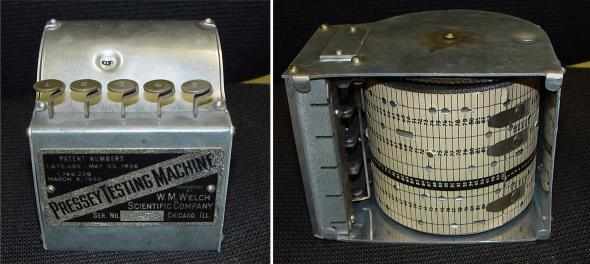
\includegraphics[scale=0.7]{imagens/pressey}
	\end{center}
	\legend{Fonte: \citeonline{pressey}}
	\label{fig:pressey}
\end{figure}

O uso da expressão ``pensamento computacional'', contudo, tem uma origem mais recente. O seu primeiro registro é observado no livro \textit{Mindstorms: Children, computers and powerful ideas}, da década de 1980, onde Seymour Papert discorre sobre a oportunidade trazida por computadores para o ensino de matemática. 

A popularização da expressão e o consequente interesse da comunidade acadêmica veio apenas com a publicação do artigo por \citeonline{wing2006}, no qual é proposto ``um conjunto de atitudes e habilidades universalmente aplicáveis'' assentadas na forma como cientistas da computação e programadores resolvem problemas.

Apesar do intenso debate despertado pelo artigo e do reconhecimento das questões e oportunidades educacionais implicadas no tema, o desenvolvimento de atividades e abordagens para sala de aula tem sido especialmente desafiador em face da parcial ou completa inexistência de um significado consensual para o conceito que seja adequado para este ambiente. A definição para o pensamento computacional resultante da discussão proposta por \citeonline{wing2006} foca apenas na contribuição da ciência da computação para as várias áreas da atividade humana, e acaba por não demonstrar como esse conceito deve se realizar no plano educacional.

Essa indefinição tem tornado difícil o estabelecimento de formas mensuráveis de avaliar o progresso dos alunos e tem redundado na inviabilização do desenvolvimento de um currículo, e consequentemente, na oferta de treinamento de professores.

Na tentativa de preencher essa lacuna, um número significativo de conferências e congressos tem sido realizado ao redor do mundo, em especial nos Estados Unidos e na Europa, financiados em boa parte por secretarias de educação e grandes empresas de tecnologia, como a Microsoft. Ao mesmo tempo, desde da publicação de \citeonline{wing2006}, uma quantidade expressiva de artigos reportando experimentações em sala de aula tem sido publicados. 

O ponto de convergência desses debates tem sido a busca de uma definição clara sobre o significado desse conceito para o contexto da sala de aula que ao mesmo tempo dialogue com as particularidades e dificuldades pertinentes a esse ambiente.

Dentre as questões para as quais se tem buscado resposta incluem-se \cite{Weintrop2016}: 

\begin{enumerate}
  \item Como o pensamento computacional se relaciona com as atuais disciplinas e práticas correntes em sala de aula?
  \item Como se estabeleceria a progressão de assuntos a serem trabalhados? 
  \item Quais são as práticas educacionais refletidas pelo pensamento computacional, e como preparar professores para que possam empregá-las em sala de aula? 
  \item Qual é melhor forma de avaliar o uso e o exercício dessas práticas pelos alunos?
\end{enumerate}

Alguns exemplos concretos da formulação desses e de outros questionamentos podem ser encontrados no relatório produzido pelo Conselho Nacional de Pesquisas dos Estados Unidos (NRC), resultante de um encontro realizado no ano de 2010. Nele são listados vinte habilidades e práticas identificadas com o pensamento computacional, tais como a abstração e decomposição de problemas, formulação de soluções heurísticas e de estratégias de busca, bem como conceitos pertinentes à ciência da computação, tais como processamento paralelo e uso de recursão \apud{NRC}{Weintrop2016}.


Também vale registrar o trabalho de \citeonline{Barr2011}, no qual o esforço de significar o pensamento computacional na perspectiva da sala de aula traduziu-se no mapeamento de algumas competências a disciplinas comuns à educação básica. Esse conteúdo esta disponível nas tabelas \ref{tab:barr-1} e \ref{tab:barr-2}.


\begin{table}[!htb]
  \caption{Práticas identificadas no pensamento computacional, segundo \citeonline{Barr2011},  presentes/possíveis na educação básica}
  \label{tab:barr-1}

  \begin{center}
    \begin{tabularx}{\textwidth}{@{}YYYYYY@{}}
      \hline 
      \textbf{Práticas} & \textbf{Matemática} & \textbf{Ciência} & \textbf{Estudos Sociais} & \textbf{Linguagens} \\

      \hline
      \\
      \textit{Coleta de   dados} & Encontrar fonte de dados de um problema, lançando dados ou moedas, por exemplo & Recolhimento de dados de um
      experimento & Estudar estatísticas de batalha ou outras estatísticas populacionais & Fazer uma análise linguística
      de sentenças. \\ \\

      \hline
      \\
      \textit{Análise de dados} & Contagem da ocorrências de lançamentos de moeda ou dados e analisar resultados & Analisar os dados a partir de um experimentar & Identificar tendências nos dados a partir de estatísticas & Identificar padrões para frase de diferentes tipos. \\ \\
      
      \hline
      \\
      \textit{ Representação de dados} & Use histograma, gráfico circular, gráfico de barras... Usar conjuntos, listas, gráficos, etc. & Resumir dados de um experimento & Resumir e representam tendências & Representar padrões de diferentes tipos de sentença \\ \\

      \hline
      \\
      \textit{Decomposição de problemas} & Aplicar ordem de operações em uma
      expressão & Fazer classificação de espécies & - & Escrever um esboço \\ \\ 

      \hline
      \\
      \textit{Abstração} & User variáveis em álgebra; estudar funções algébricas em comparação com as funções na programação & Construir um modelo de uma entidade física & Resumir os fatos; deduzir conclusões a partir de factos & - \\ \\% 
      \hline
    \end{tabularx}
  \end{center}
  \legend{Fonte: Adaptado de \citeonline{Barr2011}}
\end{table}

\begin{table}[!htb]
  \caption{\textit{Continuação} - Práticas identificadas no pensamento computacional, segundo \citeonline{Barr2011}, presentes/possíveis na educação básica}
  \label{tab:barr-2}
  \begin{center}
    \begin{tabularx}{\textwidth}{@{}YYYYYY@{}}
      \hline 
      
      \textbf{Práticas} & \textbf{Matemática} & \textbf{Ciências} & \textbf{Estudos Sociais} & \textbf{Linguagens} \\

      \hline
      \\
      \textit{Procedimentos algorítmicos} & Longa divisão, fatoração & Fazer procedimentos experimentais & - & Escrever instruções \\ \\ % 

      \hline
      \\
      \textit{Automação} & - & Usar \textit{Probware} ou \textit{Origin} & Usar excel & Usar um corretor ortográfico \\ \\ 

      \hline
      \\
      \textit{Paralelização} & Resolver sistema lineares; fazer multiplicação de matrizes & Executar simultaneamente experimentos com diferentes parâmetros & - & - \\ \\

      \hline
      \\
      \textit{Simulação} & Representar graficamente uma função em um plano cartesiano e modificar os valores da variáveis & Simular o movimento de o sistema solar & Jogar Age of Empires; Trilha de Oregon & Fazer uma reencenação de uma história \\ \\
      \hline

    \end{tabularx}
  \end{center}
  \legend{Fonte: Adaptado de \citeonline{Barr2011}}
\end{table}

Outro trabalho merecedor de registro é o de \citeonline{Brennan2012}. Nele o pensamento computacional é trabalhado sob a perspectiva da aprendizagem de programação e é estruturado em três dimensões: 

\begin{enumerate}
\item \textbf{conceitos computacionais} - conceitos com os quais os estudantes se envolvem ao aprender a programar, tais como iteração e paralelismo.

\item \textbf{práticas computacionais} - práticas que os estudantes desenvolvem quando se engajam com esses conceitos.

\item \textbf{perspectivas computacionais} - perspectivas que os estudantes adquirem sobre o mundo ao seu redor e sobre si mesmo, resultantes desse aprendizado.
\end{enumerate}

Acompanhando essa proposta, são sugeridas formas de avaliar o progresso dos alunos em cada uma delas. O uso do ambiente \textit{Scratch}, ilustrado na figura \ref{fig:scratch}, desenvolvido pelo \textit{MIT Labs}, marca o desenvolvimento do artigo.

\begin{figure}[!htb]
	\caption{\textit{Scratch} - linguagem de programação visual desenvolvido pelo \textit{MIT Labs}.}
  \begin{center}
	  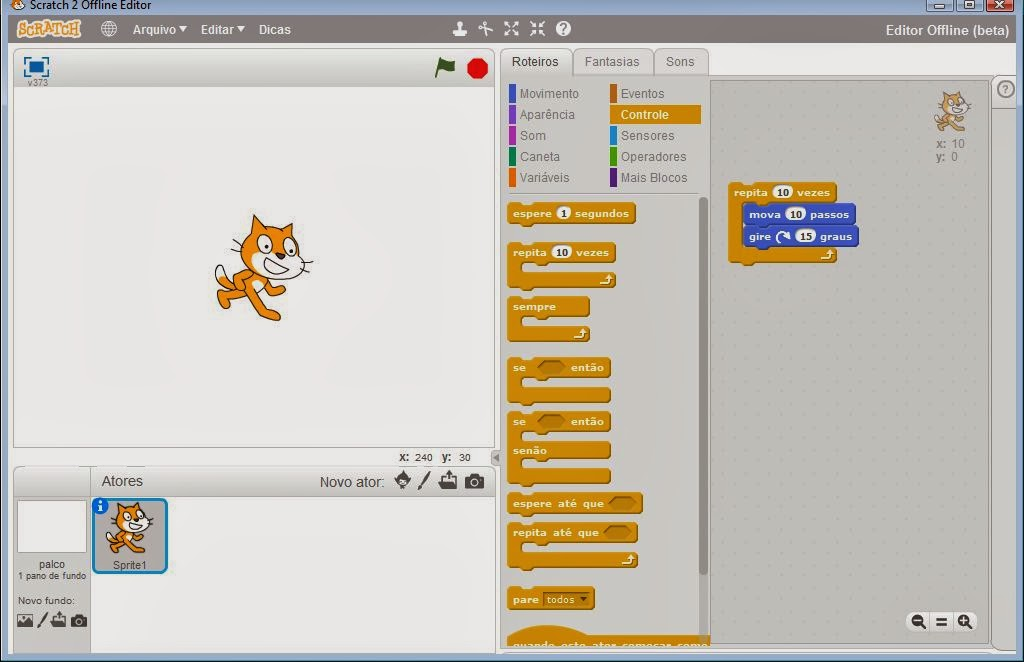
\includegraphics[max width=\textwidth]{imagens/scratch}
	\end{center}
	\label{fig:scratch}
\end{figure}

Ao longo das páginas seguintes, iremos apoiar as nossas análises na proposição de \citeonline{Weintrop2016}. Entre os trabalhos analisados, esta contribuição é a que melhor responde à nossa necessidade de oferecer uma perspectiva prática do pensamento computacional, coerente com as necessidades do ensino de ciências. Isso porque nele podemos observar a delimitação clara das competências a serem exercitadas pelos alunos e como elas tendem a favorecer a tão almejada aprendizagem científica.

Essa definição é alcançada pela criação de uma taxonomia que contemple as principais práticas identificadas pelo autor que estão relacionadas ao pensamento computacional. Na seção seguinte iremos detalha-la, mas, previamente, descrever a metodologia adotada. E como definições só podem ser úteis se forem acompanhada de exemplos práticos, iremos, em seguida, demonstrar como o exercício dessas competências podem ser incorporadas a temas das aulas de ciências, ao mesmo tempo que ilustramos a discussão com a descrição de casos reais.

\section{A criação de uma taxonomia para o pensamento computacional}

A definição de uma taxonomia segue na esteira dos empreendimentos cujo objetivo tem sido uma significação funcional para o pensamento computacional. Nas palavras de \citeonline{Weintrop2016}, o que se busca é 

\begin{citacao}
$[...]$ uma abordagem diferente para a definição do pensamento computacional, contando com a aplicação das práticas identificadas acima em contextos distintos da ciência da computação. Ao fazer isso, deixamos de confiar em ideias e práticas descontextualizadas e, em vez disso, recorremos a instanciações reais do pensamento computacional na natureza para fornecer clareza e especificidade sobre o que o termo significa. Isso reforça o argumento de que essas práticas são amplamente aplicáveis, ao mesmo tempo em que fornecem uma definição concreta e acionável do pensamento computacional. \cite[Tradução nossa]{Weintrop2016}
\end{citacao}

A metodologia adotada envolveu o emprego de três recursos básicos:

\begin{enumerate}
  \item amostras de atividades educativas envolvendo pensamento computacional tanto em matemáticas como em ciências.
  \item levantamento de conceitos existentes sobre o pensamento computacional presentes na literatura.
  \item entrevistas com matemáticos e cientistas.
\end{enumerate}

Os passos dados pelos autores foram assim sequenciados:

\begin{enumerate}
  \item \textbf{Delimitação das rotinas e habilidades relacionadas.} Com o objetivo de identificar as competências e práticas que são associadas repetidamente ao pensamento computacional, uma revisão da literatura foi feita. Dentre o material analisado estiveram tanto documentações oficiais produzidas sobre pensamento computacional, como o já citado \citeonline{NRC}, como ementas curriculares de programas de engenharia e ciência da computação. Durante essa investigação, buscou-se a aquisição de uma visão panorâmica sobre o tema antes da delimitação do escopo da análise para as disciplinas matemáticas e científicas. Dessa etapa, dez competências básicas foram extraídas (Tabela \ref{tab:ten-skills}).

  
\begin{table}[htb]
  \caption{Competências associadas ao pensamento computacional segundo análise da literatura feita por \citeonline{Weintrop2016}}
  \label{tab:ten-skills}

  \begin{center}
    \begin{tabularx}{\textwidth}{XX}
      \hline
      \\
      1. Capacidade para lidar com problemas abertos & 6. Criar abstrações para aspectos do problema em mãos 
      \\
      
      \\
      3. Persistência para trabalhar com problemas desafiadores & 7. Reestruturar um problema em termos de outros conhecidos 
      \\

      \\
      3. Confiança para lidar com a complexidade & 8. Avaliar pontos fortes/fracos de uma representação de dados/sistema representacional
      \\

      \\
      3. Representar ideas the forma computacionalmente significativa & 9. Gerar soluções algorítmicas
      \\

      \\
      3. Quebrar problemas grandes em problemas menores & 10. Reconhecer e lidar com a ambiguidade em algoritmos
      \\\\
      \hline
    \end{tabularx}
  \end{center}
  \legend{Fonte: \citeonline{Weintrop2016}}
\end{table}


  \item \textbf{Coleção e classificação de atividades voltadas para a introdução do tema nas aulas de ciências e matemática.} Foram analisadas trinta planos de aulas de uma coleção, permeadas por conteúdos de física, astronomia, química, biologia, ciências da terra, redes e programação. Todo material analisado tinha origem no programa ``Reach for Stars''\footnote{Mais informações sobre o programa pode ser encontrado em \href{http://gk12.ciera.northwestern.edu/}{http://gk12.ciera.northwestern.edu/}, } cujo propósito é a integração entre estudantes de pós-graduação de disciplinas STEM, dependentes do uso de computação nas suas pesquisas, e alunos da educação básica. Tendo como meta a identificação de práticas relacionadas às que foram recortadas do primeiro passo, uma analise foi feita por dois pesquisadores independentes. Dela emergiram um conjunto de 208 facetas do pensamento computacional, das quais uma pequena amostra é exposta na tabela \ref{tab:facetas}.
  
  \begin{table}[!htb]
  \caption{\textit{Continuação} - Práticas identificadas no pensamento computacional, segundo \citeonline{Barr2011}, presentes/possíveis na educação básica}
  \label{tab:facetas}
  \begin{center}
    \begin{tabularx}{\textwidth}{@{}YYYYYY@{}}
      \hline 
      
      \textbf{Práticas} & \textbf{Matemática} & \textbf{Ciências} & \textbf{Estudos Sociais} & \textbf{Linguagens} \\

      \hline
      \\
      \textit{Procedimentos algorítmicos} & Longa divisão, fatoração & Fazer procedimentos experimentais & - & Escrever instruções \\ \\ % 

      \hline
      \\
      \textit{Automação} & - & Usar \textit{Probware} ou \textit{Origin} & Usar excel & Usar um corretor ortográfico \\ \\ 

      \hline
      \\
      \textit{Paralelização} & Resolver sistema lineares; fazer multiplicação de matrizes & Executar simultaneamente experimentos com diferentes parâmetros & - & - \\ \\

      \hline
      \\
      \textit{Simulação} & Representar graficamente uma função em um plano cartesiano e modificar os valores da variáveis & Simular o movimento de o sistema solar & Jogar Age of Empires; Trilha de Oregon & Fazer uma reencenação de uma história \\ \\
      \hline

    \end{tabularx}
  \end{center}
  \legend{Fonte: Adaptado de \citeonline{Barr2011}}
\end{table}

\begin{table}[htbp]
  %  \centering does nothing if table is full width
    \caption{Add caption}
      \begin{tabularx}{\textwidth}{@{}YYYYYY@{}}
      % \begin{tabularx}{\textwidth}{*{3}{>{\centering\arraybackslash}X}}
      \toprule
      \textbf{Aditivo} & \multicolumn{2}{c}{\textbf{Quantidade (g)}}\\
      \cmidrule{2-3}
       & \multicolumn{2}{c}{Carga Mineral (\%)} \\
       & 20    & 30 \\
       \midrule
      \multirow{3}{*}{Fibra} & 1,266 & 252 \\
      % GCC & 0,316 & 52 \\
      % Amido & 0,016 & 25 \\
      % ASA & 0,002 & 252 \\
      % Percol & 0,00032 & 25 \\
      \bottomrule
      \end{tabularx}
    \label{tab_formacao_folhas}%
  \end{table}

  \begin{tabular}{|l|l|l|l|}\hline
    \multirow{10}{*}{numeric literals} & \multirow{5}{*}{integers} & in decimal & \verb|8743| \\ \cline{3-4}
    & & \multirow{2}{*}{in octal} & \verb|0o7464| \\ \cline{4-4}
    & & & \verb|0O103| \\ \cline{3-4}
    & & \multirow{2}{*}{in hexadecimal} & \verb|0x5A0FF| \\ \cline{4-4}
    & & & \verb|0xE0F2| \\ \cline{2-4}
    & \multirow{5}{*}{fractionals} & \multirow{5}{*}{in decimal} & \verb|140.58| \\ \cline{4-4}
    & & & \verb|8.04e7| \\ \cline{4-4}
    & & & \verb|0.347E+12| \\ \cline{4-4}
    & & & \verb|5.47E-12| \\ \cline{4-4}
    & & & \verb|47e22| \\ \cline{1-4}
    \multicolumn{3}{|l|}{\multirow{3}{*}{char literals}} & \verb|'H'| \\ \cline{4-4}
    \multicolumn{3}{|l|}{} & \verb|'\n'| \\ \cline{4-4}          %% here
    \multicolumn{3}{|l|}{} & \verb|'\x65'| \\ \cline{1-4}        %% here
    \multicolumn{3}{|l|}{\multirow{2}{*}{string literals}} & \verb|"bom dia"| \\ \cline{4-4}
    \multicolumn{3}{|l|}{} & \verb|"ouro preto\nmg"| \\ \cline{1-4}          %% here
  \end{tabular}
  
  \begin{tabular}{|l|l|l|l|}\hline
    \multirow{10}{*}{numeric literals} & \multirow{5}{*}{integers} & in decimal & \verb|8743| \\ \cline{3-4}
    && \multirow{2}{*}{in octal} & \verb|0o7464| \\ \cline{4-4}
    & & & \verb|0O103| \\ \cline{3-4}
    & & \multirow{2}{*}{in hexadecimal} & \verb|0x5A0FF| \\ \cline{4-4}
    & & & \verb|0xE0F2| \\ \cline{2-4}
    & \multirow{5}{*}{fractionals} & \multirow{5}{*}{in decimal} & \verb|140.58| \\ \cline{4-4}
    & & & \verb|8.04e7| \\ \cline{4-4}
    & & & \verb|0.347E+12| \\ \cline{4-4}
    & & & \verb|5.47E-12| \\ \cline{4-4}
    & & & \verb|47e22| \\ \cline{1-4}
    & \multicolumn{2}{l|}{\raisebox{-\totalheight}{
    %  \begin{figure}
      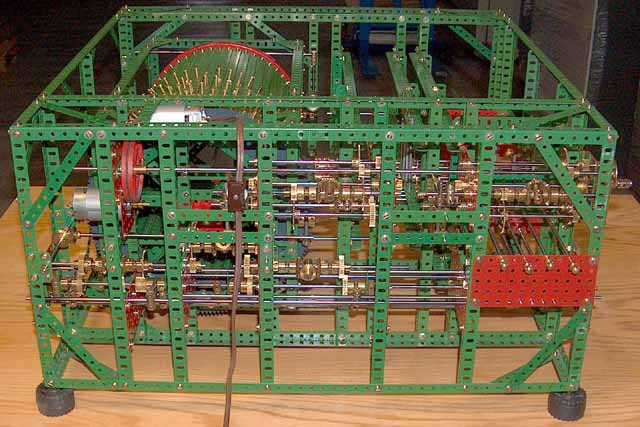
\includegraphics[width=0.3\textwidth]{imagens/babbage.jpg}
      
      % \end{figure}
      }
      } 
    % \raisebox{-\totalheight}{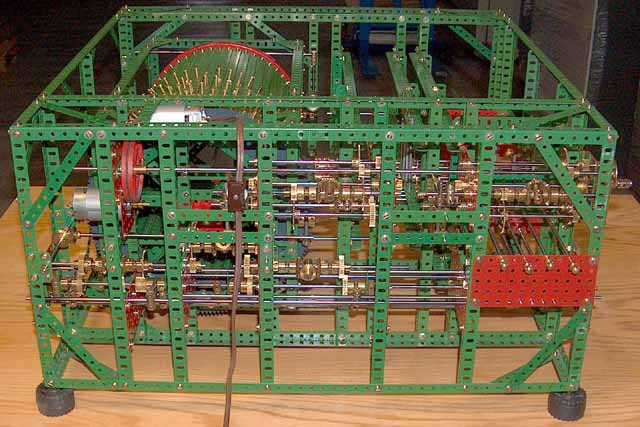
\includegraphics[width=0.3\textwidth, height=60mm]{imagens/babbage.jpg}}\\\\\cline{1-4}

    % \mutirow{4}{*}{
    % } \\ \cline{1-4}
  \end{tabular}

  \item \textbf{Organização temática.} A partir da análise feita até então, foi produzida uma lista com vinte e sete práticas, tematicamente organizada em cinco grandes campos: dados e informações, modelagem e simulação, resolução de problemas, pensamento sistêmico.

  \item \textbf{Validação} A taxonomia criada, disponível até a execução dessa etapa, foi apresentada a professores da educação básica. Com esse material em mãos, colaborativamente, eles puderam desenhar atividades para suas turmas. 

  No geral, de acordo com o autor, o \textit{feedback} fornecidos por eles foram bastante positivos, embora algumas preocupações tenham sido evidenciadas em relação às seções da taxonomia com conceitos computacionais, tais como aplicação de lógica condicional e uso de recursão e iteração. 
  
  A razão para esse receio era a percepção que tais tópicos estavam muito distantes do conteúdo trabalhado em sala de aula.

  Além de profissionais da educação básica, outros tantos \textit{feedbacks} foram colhidos com pesquisadores de alguns setores da indústria, bioquímicos, físicos, engenheiro de materiais, astrofísicos, cientistas da computação e engenheiros biomédicos.

  Além da intenção de colher avaliações, o objetivo dessa rodada de entrevistas foi a obtenção de informações e \textit{insights} sobre o como o pensamento computacional integra autênticos ambientes de pesquisas. Ao mesmo tempo, buscou-se observar as semelhanças e diferenças na forma como o uso computação se efetiva na rotina de trabalho em cada uma das áreas desses profissionais.

  \item \textbf{Revisão.} A partir dos \textit{feedbacks} e sugestões feita pelos professores e pesquisadores, uma revisão da primeira versão da taxonomia foi feita.
\end{enumerate}


O resultado final desse processo pode ser visto na tabela disponível na figura \ref{fig:taxonomia}. Uma discussão sobre cada um dos elementos dessa classificação é feita a seguir.

\begin{landscape}
  \begin{center}
    \begin{figure}[!htb]
      \caption{Taxonomia para práticas do pensamento computacional}
      \begin{center}
          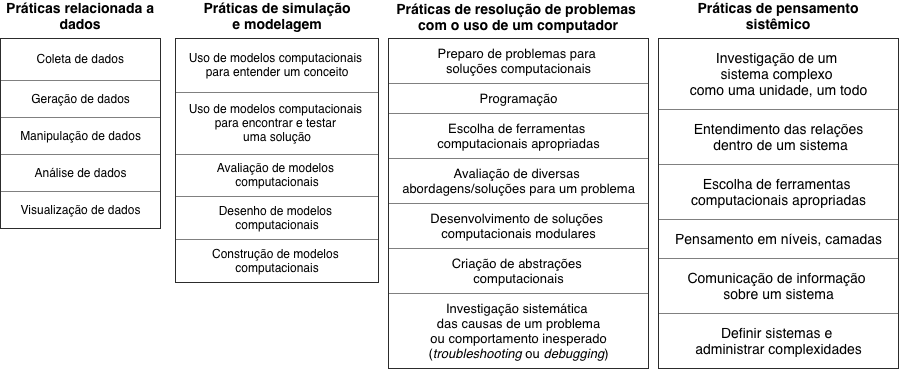
\includegraphics[scale=0.7]{imagens/taxonomia}
      \end{center}
      \legend{Fonte: \citeonline{Weintrop2016}}
      \label{fig:taxonomia}
    \end{figure}
  \end{center}
\end{landscape}

\subsection{Práticas relacionadas a dados}

\citeonline{Weintrop2016} sustenta que a capacidade de analisar e extrair significado de um grande volume de dados desestruturados tem sido uma das características definidoras da prática científica moderna. A maneira como esse empreendimento vem sendo conduzido tem sido impactados significativamente pelos avanços tecnológicos em curso. 

Para ilustrar a relevância dessa prática, o autor destaca uma das entrevistas feitas durante a elaboração da taxonomia na qual um cientista de materiais, questionado sobre como era sua pesquisa, responde: ``Em quase tudo, o que se tem são dados brutos''. Em seguida ele prossegue explicando como ele define as perguntas a serem respondidas (problemas de pesquisa), e como dados são gerados, processados e organizados, para que então, finalmente, o uso de determinados softwares gerem as visualizações para suas conclusões. 


Segundo o autor, abrigar algumas dessa práticas nas atividades escolares deve significar ajudar o alunos a perceberem que inerentemente dados não oferecem respostas imediatas, e que para alcançá-las ``ordem deve ser imposta''. Por esse motivo a introdução de noções básicas de estatística e probabilidade se faz necessária.

Cada um dos aspectos relevantes ao uso de dados são destrinchados a seguir.


\begin{enumerate}
  \item \textbf{Coleta de dados}

  O papel que os computadores cumprem na coleta de dados guarda relação com a necessidade de automatizar protocolos de registro e armazenamento de dados gerados pela observação de um fenômeno.
  
  De acordo com \citeonline{Weintrop2016}, o aluno que dominar esta prática será capaz de propor  protocolos de coleta dados e formas de uso de ferramentas computacionais que automatizam essa tarefa.

  \item \textbf{Geração de dados}
  
  Em astronomia, para a compreensão da evolução de uma galáxia, torna-se necessário a geração de dados a partir de simulações computacionais, dado que escala de tempo investigada (bilhões de anos) é incompatível com a dos pesquisadores.

  Esse exemplo ilustra um dos aspectos da pesquisa científica onde a necessidade de geração de dados impõe-se em razão de restrições circunstanciais.

  Como assinala o autor, o estudante que dominar esta prática será capaz de definir procedimentos computacionais e executar simulações que permitam a criação de dados, cuja utilização pode auxiliá-lo a aprofundar a compreensão em um tópico sob investigação.

  \item \textbf{Manipulação de dados}

  O uso de computadores torna possíveis a manipulação de dados desestruturados, de tal modo a permitir que significados possam  ser extraídos. 

  Dentre as várias técnicas existentes de manipulação, o autor cita o ordenamento, a filtragem, limpeza, normalização e união de conjunto de dados dissociados. 
  
  Como destaca, o aluno que dominar esta prática será capaz de, a partir do uso de ferramentas computacionais, remodelar um conjunto de dados de tal modo a facilitar seu trabalho de investigação.

  \item \textbf{Análise de dados}

  Em face da abundância de dados existentes, o uso de ferramentas computacionais para análise de dados tem sido um das tarefas mais relevantes da prática científica.   
  
  Dentre as várias estratégias existentes, o autor destaca a busca por padrões ou anomalias, a definição de regras para categorização de dados, e a identificação de tendências e correlações. 

  Conforme sublinha, o aluno que dominar esta prática será capaz de fazer afirmações e extrair conclusões a partir da análise de um conjunto de dados.


  \item \textbf{Visualização de dados}

  Outros aspectos relevantes e necessários da atividade científica são a comunicação e o compartilhamento de dados.

  Nesse sentido, o uso de ferramentas computacionais que tornam possível a projeção de dados, seja na forma de um gráfico simples ou de uma exposição dinâmica que permite a interação do usuário com a informação, desempenha papel preponderante.

  Conforme sustenta \citeonline{Weintrop2016}, o aluno que dominar esta prática será capaz de usar com eficiência ferramentas de visualização que permitam a comunicação de informações e conclusões extraídas durante a análise.

\end{enumerate}

\section{Práticas de simulação e modelagem}

Outro conjunto práticas que compõe a taxonomia de \citeonline{Weintrop2016} são aquelas relacionadas ao exercício da representação de fenômenos, também presentes no uso e criação de modelos e simulacros computacionais. 

Falando especificamente de modelos, podemos dizer que eles ``todos estão errados, mas alguns deles são úteis'' \apud{box1987empirical}{Weintrop2016}, dado o caráter simplificador, mas representativo de alguns - proporcional à capacidade descritiva e preditiva que comportam. 

Dentre as várias formas que um modelo pode assumir, o autor destaca os fluxogramas, os diagramas, as equações, as fórmulas químicas, os modelos físicos (como maquetes ou representações tridimensionais de uma molécula), e por fim os modelos computacionais - representações não-estáticas de um fenômeno que podem ser simuladas por um computador \cite{Weintrop2016}.

\begin{figure}[!htb]
  \caption{Modelo físico de uma cadeia de DNA}
	\begin{center}
    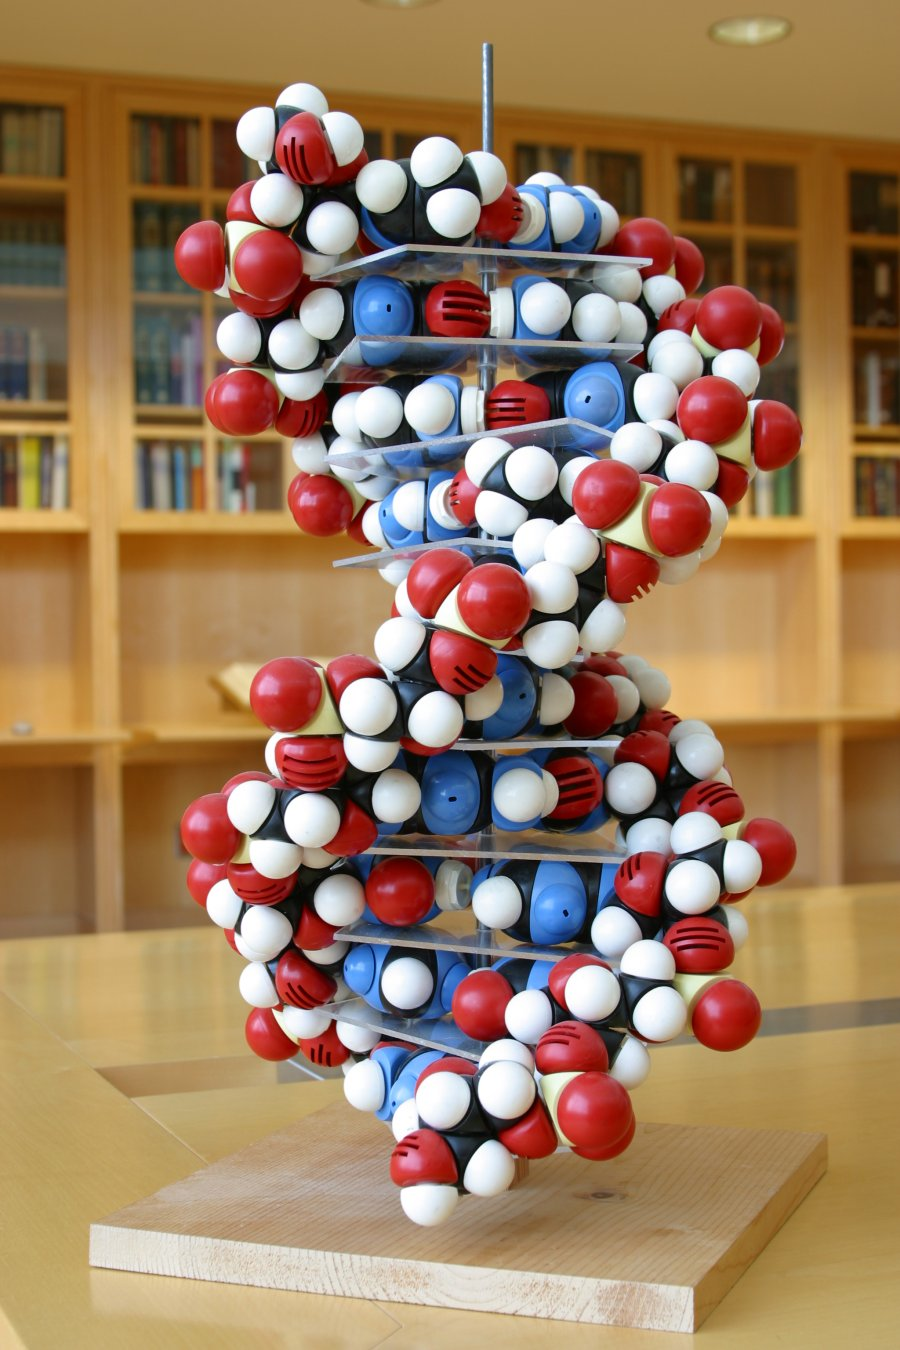
\includegraphics[width=0.5\textwidth]{imagens/modelo_fisico.jpg}
	\end{center}
	\label{fig:modelo-fisico}
\end{figure}
% O autor traz algumas definições que tornam mais nítidas a relevância desses elementos de representação. 

De um ponto de vista pedagógico, como ressalta o autor, a utilidade de modelos e simulações computacionais está na possibilidade de tornar a compreensão de um fenômeno mais clara e permitir a investigação de comportamentos cuja condições determinantes são difíceis, senão impossíveis de reproduzir.

O poder didático dessas ferramentas, contudo, não está apenas no seu uso, mas na possibilidade do estudante também criá-las, tornando possível a formulação de suas próprias interpretações. 

Como ressalta \citeonline{Weintrop2016}, os educadores reconhecem que tais práticas de representação são indissociáveis da aprendizagem científica, mas elas são raremente explicitadas como parte da instrução. E é exatamente para contornar esse problema que novas formulações curriculares tem tornado claro a necessidade de estimular a criação, e não apenas o uso de modelos acabados. 

Abaixo listamos as cinco práticas incluídas na taxonomia, referentes à simulação e modelagem.

\begin{enumerate}
  \item \textbf{Uso de modelos computacionais para entender um conceito}

  Segundo o autor, o uso de modelos computacionais que demonstram ideias específicas ou simulam comportamento de fenômenos são poderosas ferramentas didáticas.

  Isso porque eles tendem a oferecer suporte a investigações sistemáticas que permitem o exercício do controle sobre parâmetros de comportamento, através de combinações e variações que, normalmente, são difíceis, senão impossíveis, de reproduzir sem o aparato computacional.

  Por isso, conclui que o estudante que dominar essa prática será capaz de aprofundar sua compreensão sobre um fenômeno ou conceito sob investigação, utilizando modelos computacionais que os reproduzem.

  \item \textbf{Uso de modelos computacionais para encontrar e testar uma solução}
  



  \item \textbf{Avaliação de modelos computacionais}

  A capacidade de avaliar a relação de um modelo computacional com a realidade representada é um dos aspectos aspectos essenciais para medirmos a sua adequabilidade, segundo \citeonline{Weintrop2016}.

  O autor aponta algumas questões que precisam ser analisadas e respondidas quando se tem esse fim em mente. Dentre elas estão as seguintes:

  \begin{enumerate}
    \item Quais suposições que os criadores do modelo fizeram sobre o mundo e como elas afetam o seu comportamento?
    \item Quais as camadas de abstração foram incorporadas ao modelo e como elas moldam a fidelidade da sua representação do fenômeno?
    \item Quais são os aspectos do modelo que foram fielmente modelados e quais outros foram simplificados ou simplesmente ignorados?
  \end{enumerate}

  Responder essas questões é tarefa essencial para compreensão dos limites de uma representação. Ao mesmo tempo, tê-las em contas é fundamental para que se possa validá-la ou não.

  De acordo com o autor, o aluno que dominar esta prática ``será capaz de articular as diferenças entre o modelo e fenômeno representado, o que inclui o levantamento de ameças a sua validade e a identificação das suposições que o sustentam'' \cite{Weintrop2016}.

  \item \textbf{Desenho de modelos computacionais}
  O desenho de modelos computacionais podem ser norteados por algumas motivações. Dentre as já discutidas, podemos citar a necessidade de testar hipóteses ou comunicar ideas, e o interesse em compreender melhor um fenômeno, 

  Durante esse processo somos levados a tomada de algumas decisões, que podem variar de acordo com o problema a ser resolvido. Dentre as mais recorrentes, \citeonline{Weintrop2016} cita a necessidade de definir os limites do sistema - explicitar aquilo que deve ser incorporado e/ou descartado - e conceitualizar as propriedades e comportamentos dos elementos incluídos. Ao final, deve ser assegurado que o produto resultante atende aos objetivos que inicialmente motivaram a construção do modelo \cite{Weintrop2016}.

  Portanto, os estudantes que exercitarem essa prática terão a oportunidade de desenhar modelos computacionais, descrevendo-os e decidindo quais dados serão produzidos, enquanto poderão cultivar o hábito de fazer avaliações críticas, a partir da análise dos limites da representação, das suposições nela incorporadas. Espera-se que com essa reflexão eles possam entender a extensão das conclusões que podem ser extraídas do modelo.

   
  

  \item \textbf{Construção de modelos computacionais}
  
\end{enumerate}



% Diante da urgência e para estruturar o curriculo de ciências em torno pensamento

% Dentre as várias soluções para inserção do pensamento computacional, nascidas da necessidade de estrutura





% Apoiado em algumas delas \citeonline{Weintrop2016} propõe um conjunto de competências  

% Nas próximas seções iremos nos apoiar em alguma delas para responder a seguinte por

% \end{landscape}





